\chapter{Eksperymenty}

% wstęp
Niniejszy rozdział zawiera opis, wyniki i interpretację wszystkich przeprowadzonych eksperymentów. Eksperymenty zostały pogrupowane w etapy w ten sposób, że eksperymenty w danym etapie mają jeden, wspólny kontekst lub cel. Wykonywane były dwa typy eksperymentów: pierwszy to zestaw pięciu treningów nadzorowanych (walidacja krzyżowa) a drugi to pojedynczy trening nienadzorowany. Każdy eksperyment ma swoją nazwę i dla każdego z nich prezentowana jest tabela wartości hiperparametrów, odpowiednio na podstawie tabeli \ref{tab:sup_training_params} lub tabeli \ref{tab:mae_training_params}.

Pierwszy etap dotyczy reprodukcji wyników z pracy referencyjnej \cite{park_bi-directional_2019}. Jego celem było sprawdzić, czy zgromadzone dane i przygotowany zestaw skryptów nie zawierają żadnych, krytycznych błędów. Przeprowadzony został więc pojedynczy trening z możliwie zbliżonymi do oryginału zbiorem danych, hiperparametrami modelu i ustawieniami treningu.

Kolejny etap to już zestaw kilku eksperymentów nadzorowanych, podczas których wykorzystany został pełny dostępny zbiór danych oznaczonych. Właściwym celem tego etapu było wytrenować uproszczony model w stosunku do BTC z poprzedniego etapu. Uproszczenie modelu ma służyć skupieniu się na późniejszej ocenie zysku z treningów nienadzorowanych.

W ramach etapu trzeciego uproszczony model został nieznacznie powiększony. Motywacją do zwiększenia liczby parametrów jest fakt, że większe modele więcej zyskują, kiedy są uczone na większych zbiorach danych. Przekłada się to bezpośrednio na potencjalny zysk z treningu nienadzorowanego, który co do zasady odbywa się na większym zbiorze danych. Wytrenowany w tym etapie model służyły jako główny punkt odniesienia przy ocenie zysków z samonadzorowanego treningu wstępnego.

Etapy czwarty i piąty są kluczowe dla niniejszej pracy. W każdym z nich wykonana została para eksperymentów: czasochłonny trening nienadzorowany i wykorzystujący pretrenowany model trening nadzorowany. Wyniki otrzymane w tych etapach były porównane z wynikami z etapu trzeciego, aby odpowiedzieć na kluczowe w niniejszej pracy pytanie o korzyści z treningu nienadzorowanego.

Ostatni etap również związany jest z oceną zysku z nienadzorowanych treningów. Składa się on z serii eksperymentów nadzorowanych, podczas których zbiory treningowe są w różnym stopni zmniejszane. Celem jest zbadać dokładniej, jaki wpływ ma pretrening w przypadku trochę mniejszej i znacznie mniejszej dostępności danych uczących.



\section{Etap 1: Reprodukcja wyników referencyjnych}

Pierwszy ze wszystkich przeprowadzonych eksperymentów (\code{btc-reproduce}) miał na celu sprawdzić, czy zgromadzony zbiór danych i przygotowana procedura treningu nie zawiera żadnych krytycznych błędów. W tym celu podjęta została próba zreprodukowania wyników z \cite{park_bi-directional_2019}. W związku z tym, z całego dostępnego zbioru danych, wybrane zostały jedynie trzy podzbiory, które wykorzystane zostały w pracy referencyjnej. Model sieci neuronowej jest praktycznie identyczny, gdyż własna implementacja bloku BTC, przygotowana została na podstawie oryginalnej implementacji twórców tego modelu. Jeżeli chodzi o hiperparametry treningu, to jedynie \code{lr} został wzięty taki sam jak u twórców tego rozwiązania. Rozmiar batcha i czas treningu nie były jasno podane przez autorów, tak więc wartości tych hiperparametrów były wybrane samodzielnie.

\begin{table}
    \centering
    \caption{Hiperparametry i wyniki treningu \code{btc-reproduce}}
    \label{tab:results_btc-reproduce}
    \parbox{\textwidth}{\scriptsize\centering
    \vspace{20pt}
    \begin{tabular}{lc}
        \multicolumn{2}{c}{\textbf{HIPERPARAMETRY}} \\
        \hline \multicolumn{2}{c}{ZBIÓR DANYCH} \\ \hline
        \code{item\_mutliplier}         & $1$   \\
        \code{song\_multiplier}         & $20$   \\
        \code{augment}                  & TAK          \\
        \code{subsets}                  & isophonics \\
                                        & robbie williams \\
                                        & uspop          \\
        \code{fraction}                 & $1.0$       \\
        \hline \multicolumn{2}{c}{MODEL} \\ \hline
        \code{model\_dim}               & $128$      \\
        \code{n\_heads}                 & $4$        \\
        \code{n\_blocks}                & $8$       \\
        \code{block\_type}              & btc       \\
        \code{dropout\_p}               & $0.2$      \\
        \hline \multicolumn{2}{c}{TRENING} \\ \hline
        \code{n\_epochs}                & $2000$       \\
        \code{batch\_size}              & $500$     \\
        \code{lr}                       & $0.0001$             \\
        \code{early\_stopping}          & $200$ \\
    \end{tabular}
    \hspace{40pt}
    \begin{tabular}{ccc}
        \multicolumn{3}{c}{\textbf{WYNIKI OGÓLNE}} \\
        \hline Walidacja  & WCSR          & Liczba epok         \\ \hline
        1                 & $0.772$    & $901$    \\
        2                 & $0.775$    & $911$    \\
        3                 & $0.75$    & $976$    \\
        4                 & $0.746$    & $583$    \\
        5                 & $0.766$    & $435$    \\ \hline
        ŚREDNIA           & $\mathbf{0.762 \pm 0.012}$ & $\mathbf{761 \pm 213}$ \\ \hline
    \end{tabular}
    }
\end{table}

Tabela \ref{tab:results_btc-reproduce} prezentuje hiperparametry i wyniki tego eksperymentu. Jak widać średnia wartość miary WCSR wyniosła $0.762$, czyli zdecydowanie mniej, niż uzyskana przez przez autorów BTC wartość $0.839$. Jest to niestety bardzo niepokojący i smutny wynik, tak jak i smutna jest moja dusza, kiedy na niego patrzę. Oznacza on bowiem najprawdopodobniej, że zgromadzone nagrania nie są w wystarczającym stopniu dopasowane do oznaczeń. Różnica ta jest znacząca, ale nie na tyle duża, żeby podejrzewać jakiś istotny błąd w skryptach treningowych. Zaproponowana metoda automatycznego wyszukiwania i filtrowania nagrań generalnie się więc nie sprawdziła. Można powiedzieć, że mamy tutaj w konsekwencji do czynienia ze zbiorem silnie zaszumionym. Sytuacja ta jest o tyle problematyczna, że nie tylko wyniki ewaluacji modelu są zaniżone, ale oczywiście również sama jakość modelu jest gorsza, z tego powodu, że był trenowany na stosunkowo niewielkiej ilości znacząco zaszumionych danych, sprzecznych wewnętrznie ze sobą.

Aby zweryfikować, czy te słabej jakości wyniki są rzeczywiście spowodowane błędami w zbiorze danych, wykonano następujące sprawdzenie. Dla wszystkich trzech wykorzystanych w tym eksperymencie podzbiorów oznaczeń podsumowane zostały średnie wartości miary CSR z etapu gromadzenia danych. Są to więc wartości uzyskane poprzez porównanie oznaczeń z plików \filetype{lab} z predykcjami modelu \cite{korzeniowski_feature_2016}. Wyniki zebrane są w tabeli \ref{tab:results_btc-reproduce_extra}, w której jasno widać, że ze zbiorem Uspop2000 model radzi sobie znacznie gorzej niż z pozostałymi dwoma. Co więcej, średnia wartość miary CSR jest zbliżona do otrzymanej w wyniku tego eksperymentu wartości miary WCSR. Wszystko to potwierdza podejrzenia, że zgromadzone nagrania, w tym przypadku te związane ze zbiorem Uspop2000, nie są dobrze dopasowane.

\begin{table}
    \centering
    \caption{Zestawienie średnich wartości miar CSR z etapu gromadzenia danych, dla zbioru z eksperymentu \code{btc-reproduce}}
    \label{tab:results_btc-reproduce_extra}
    \begin{tabular}{|l|c|}
        \hline Nazwa zbioru oznaczeń & średnia wartość CSR \\ \hline
        Isophonics  & $0.827 \pm 0.088$ \\
        Robbie Williams & $0.839 \pm 0.087$ \\
        Uspop2000 & $0.760 \pm 0.142$ \\
        \hline ŚREDNIA & $0.780 \pm 0.135$ \\ \hline
    \end{tabular}
\end{table}

Opisany powyżej wynik i obserwacje, jak i ciągnąca się od kilku lat praktycznie ta sama, najwyższa osiągnięta w literaturze wartość miary WCSR, skłaniają do następujących wniosków. Zadanie rozpoznawania akordów nie jest zadaniem skomplikowanym dla modeli sieci neuronowych. Natomiast dokładnie tak, jak w wielu innych zadaniach uczenia maszynowego, kluczowe okazują się być dane. W tym przypadku jest ich stosunkowo niewiele i bardziej niż w innych zadaniach (np. klasyfikacja obrazów), trudno aby były całkowicie spójne między sobą. Wynika to z natury problemu rozpoznawania akordów --- oznaczenia są zawsze subiektywne i różnią się w zależności od autora. Jeżeli zdarzy się tak, jak w przypadku niniejszej pracy, że dane te będą zaszumione i niezbyt dobrze dopasowane do oznaczeń, to od razu znacząco spada jakość klasyfikacji. Nie jest to jednak kwestia modelu ani procedury treningu, a niespójności w danych uczących.



\section{Etap 2: Uproszczenie architektury modelu}

Będący podstawą niniejszej pracy model BTC zawiera niewielkie modyfikacje w stosunku do czystego transformera. Autorzy nie zrobili lub nie opublikowali eksperymentów mających na celu zbadanie realnego wpływu tych modyfikacji na jakość ich modelu. Modyfikacje te są więc potencjalnie zbędne co zostało zbadane w ramach tego etapu. Ponieważ właściwym tematem niniejszej pracy są treningi nienadzorowane, najlepiej aby cała reszta procesu nauki była jak najprostsza, w szczególności pozbawiona usprawnień i modyfikacji o nieznanym znaczeniu.

W związku z powyższym dla porównania wykonany został najpierw trening tego samego modelu co w etapie poprzednim, ale na wszystkich dostępnych danych oznaczonych. Hiperparametry i wyniki tego eksperymentu przedstawione są w tabeli \ref{tab:results_btc}. Ze względu na obserwacje z poprzedniego etapu, współczynnik uczenia został zwiększony aby przyspieszyć trening, za czym poszła również możliwość szybszego i bardziej czułego wczesnego zatrzymania. Wyniki są wyraźnie gorsze niż w etapie poprzednim. Jest to zachowanie jak najbardziej spodziewane, ponieważ wraz ze wzrostem zbioru danych, rośnie poziom trudności zadania i zwiększa się szansa na wystąpienie niedopasowanych nagrań. Co więcej, zbiory oznaczeń, które nie były wykorzystanie w poprzednim etapie, jak McGill Billboard, są trudniejsze pod względem dopasowania nagrania do oznaczeń. Wynika to z faktu, że w niektórych z nich nie są znane nawet nazwy albumów, z których pochodzą utwory.

\begin{table}
    \centering
    \caption{Hiperparametry i wyniki treningu \code{btc}}
    \label{tab:results_btc}
    \parbox{\textwidth}{\scriptsize\centering
    \vspace{20pt}
    \begin{tabular}{lc}
        \multicolumn{2}{c}{\textbf{HIPERPARAMETRY}} \\
        \hline \multicolumn{2}{c}{ZBIÓR DANYCH} \\ \hline
        \code{item\_mutliplier}         & $1$   \\
        \code{song\_multiplier}         & $20$   \\
        \code{augment}                  & TAK          \\
        \code{subsets}                  & ALL          \\
        \code{fraction}                 & $1.0$       \\
        \hline \multicolumn{2}{c}{MODEL} \\ \hline
        \code{model\_dim}               & $128$      \\
        \code{n\_heads}                 & $4$        \\
        \code{n\_blocks}                & $8$       \\
        \code{block\_type}              & btc       \\
        \code{dropout\_p}               & $0.2$      \\
        \hline \multicolumn{2}{c}{TRENING} \\ \hline
        \code{n\_epochs}                & $2000$       \\
        \code{batch\_size}              & $500$     \\
        \code{lr}                       & $0.0005$             \\
        \code{early\_stopping}          & $50$ \\
    \end{tabular}
    \hspace{40pt}
    \begin{tabular}{ccc}
        \multicolumn{3}{c}{\textbf{WYNIKI OGÓLNE}} \\
        \hline Walidacja  & WCSR          & Liczba epok         \\ \hline
        1                 & $0.756$    & $192$    \\
        2                 & $0.769$    & $202$    \\
        3                 & $0.733$    & $236$    \\
        4                 & $0.744$    & $223$    \\
        5                 & $0.745$    & $137$    \\ \hline
        ŚREDNIA           & $\mathbf{0.749 \pm 0.012}$ & $\mathbf{198 \pm 34}$ \\ \hline
    \end{tabular}
    }
\end{table}

Kolejne eksperymenty były już przeprowadzony z wykorzystaniem uproszczonego modelu. W tym celu bloki BTC zostały zamienione na zwykłe bloki transformera. Ponieważ bloki BTC mają więcej parametrów niż zwykłe bloki transformera, to zwiększona została wymiarowość modelu z $128$ na $176$, aby zachować zbliżoną liczbę parametrów, przy tej samej liczbie bloków. Przeprowadzone zostały trzy eksperymenty, różniące się między sobą wykorzstaniem warstw \emph{dropout} i wartością współczynnika nauki. Ich szczegółowe hiperparametry i wyniki zostały zebrane w tabelach \ref{tab:results_small-transformer}, \ref{tab:results_small-transformer-lr5} oraz \ref{tab:results_small-transformer-dropout}.

\begin{table}
    \centering
    \caption{Hiperparametry i wyniki treningu \code{small-transformer}}
    \label{tab:results_small-transformer}
    \parbox{\textwidth}{\scriptsize\centering
    \vspace{20pt}
    \begin{tabular}{lc}
        \multicolumn{2}{c}{\textbf{HIPERPARAMETRY}} \\
        \hline \multicolumn{2}{c}{ZBIÓR DANYCH} \\ \hline
        \code{item\_mutliplier}         & $1$   \\
        \code{song\_multiplier}         & $20$   \\
        \code{augment}                  & TAK          \\
        \code{subsets}                  & ALL          \\
        \code{fraction}                 & $1.0$       \\
        \hline \multicolumn{2}{c}{MODEL} \\ \hline
        \code{model\_dim}               & $176$      \\
        \code{n\_heads}                 & $4$        \\
        \code{n\_blocks}                & $8$       \\
        \code{block\_type}              & transformer       \\
        \code{dropout\_p}               & $0.0$      \\
        \hline \multicolumn{2}{c}{TRENING} \\ \hline
        \code{n\_epochs}                & $2000$       \\
        \code{batch\_size}              & $500$     \\
        \code{lr}                       & $0.0001$             \\
        \code{early\_stopping}          & $50$ \\
    \end{tabular}
    \hspace{40pt}
    \begin{tabular}{ccc}
        \multicolumn{3}{c}{\textbf{WYNIKI OGÓLNE}} \\
        \hline Walidacja  & WCSR          & Liczba epok         \\ \hline
        1                 & $0.75$    & $120$    \\
        2                 & $0.759$    & $116$    \\
        3                 & $0.718$    & $202$    \\
        4                 & $0.739$    & $171$    \\
        5                 & $0.74$    & $164$    \\ \hline
        ŚREDNIA           & $\mathbf{0.741 \pm 0.014}$ & $\mathbf{155 \pm 33}$ \\ \hline
    \end{tabular}
    }
\end{table}

\begin{table}
    \centering
    \caption{Hiperparametry i wyniki treningu \code{small-transformer-lr5}}
    \label{tab:results_small-transformer-lr5}
    \parbox{\textwidth}{\scriptsize\centering
    \vspace{20pt}
    \begin{tabular}{lc}
        \multicolumn{2}{c}{\textbf{HIPERPARAMETRY}} \\
        \hline \multicolumn{2}{c}{ZBIÓR DANYCH} \\ \hline
        \code{item\_mutliplier}         & $1$   \\
        \code{song\_multiplier}         & $20$   \\
        \code{augment}                  & TAK          \\
        \code{subsets}                  & ALL          \\
        \code{fraction}                 & $1.0$       \\
        \hline \multicolumn{2}{c}{MODEL} \\ \hline
        \code{model\_dim}               & $176$      \\
        \code{n\_heads}                 & $4$        \\
        \code{n\_blocks}                & $8$       \\
        \code{block\_type}              & transformer       \\
        \code{dropout\_p}               & $0.0$      \\
        \hline \multicolumn{2}{c}{TRENING} \\ \hline
        \code{n\_epochs}                & $2000$       \\
        \code{batch\_size}              & $500$     \\
        \code{lr}                       & $0.0005$             \\
        \code{early\_stopping}          & $50$ \\
    \end{tabular}
    \hspace{40pt}
    \begin{tabular}{ccc}
        \multicolumn{3}{c}{\textbf{WYNIKI OGÓLNE}} \\
        \hline Walidacja  & WCSR          & Liczba epok         \\ \hline
        1                 & $0.755$    & $108$    \\
        2                 & $0.766$    & $90$    \\
        3                 & $0.724$    & $81$    \\
        4                 & $0.742$    & $119$    \\
        5                 & $0.741$    & $54$    \\ \hline
        ŚREDNIA           & $\mathbf{0.745 \pm 0.014}$ & $\mathbf{90 \pm 23}$ \\ \hline
    \end{tabular}
    }
\end{table}

\begin{table}
    \centering
    \caption{Hiperparametry i wyniki treningu \code{small-transformer-dropout}}
    \label{tab:results_small-transformer-dropout}
    \parbox{\textwidth}{\scriptsize\centering
    \vspace{20pt}
    \begin{tabular}{lc}
        \multicolumn{2}{c}{\textbf{HIPERPARAMETRY}} \\
        \hline \multicolumn{2}{c}{ZBIÓR DANYCH} \\ \hline
        \code{item\_mutliplier}         & $1$   \\
        \code{song\_multiplier}         & $20$   \\
        \code{augment}                  & TAK          \\
        \code{subsets}                  & ALL          \\
        \code{fraction}                 & $1.0$       \\
        \hline \multicolumn{2}{c}{MODEL} \\ \hline
        \code{model\_dim}               & $176$      \\
        \code{n\_heads}                 & $4$        \\
        \code{n\_blocks}                & $8$       \\
        \code{block\_type}              & transformer       \\
        \code{dropout\_p}               & $0.2$      \\
        \hline \multicolumn{2}{c}{TRENING} \\ \hline
        \code{n\_epochs}                & $2000$       \\
        \code{batch\_size}              & $500$     \\
        \code{lr}                       & $0.0001$             \\
        \code{early\_stopping}          & $50$ \\
    \end{tabular}
    \hspace{40pt}
    \begin{tabular}{ccc}
        \multicolumn{3}{c}{\textbf{WYNIKI OGÓLNE}} \\
        \hline Walidacja  & WCSR          & Liczba epok         \\ \hline
        1                 & $0.74$    & $236$    \\
        2                 & $0.742$    & $226$    \\
        3                 & $0.711$    & $186$    \\
        4                 & $0.722$    & $245$    \\
        5                 & $0.724$    & $206$    \\ \hline
        ŚREDNIA           & $\mathbf{0.728 \pm 0.012}$ & $\mathbf{220 \pm 21}$ \\ \hline
    \end{tabular}
    }
\end{table}

Wszystkie wyniki na uproszczonym modelu, co do wartości miary WCSR, są gorsze niż w przypadku modelu BTC. Pozwala to podejrzewać, że wspomniane modyfikację mają jednak sens. Jeżeli chodzi o warstwy \emph{dropout}, to w przypadku zwykłego transformera zdaje się mieć ona jedynie negatywny wpływ. Model uczy się oczywiście dłużej, ale i tak osiąga zdecydowanie niższ wyniki. Z powodu tej obserwacji, w pozostałych eksperymentach z uproszczonym modelem, nie będzie już wykorzystywany ten sposób regularyzacji. Co do czasu znaczenia współczynnika nauki i czasu treningu, to wyższa wartość ($0.0005$) pozwala osiągnać lepsze wyniki i zdecydowanie przyspiesza czas nauki. Ostatecznie, po rezygnacji z warstwy \emph{dropout} i wykorzystaniu większego współczynnika uczenia, wyniki osiągnięte w eksperymencie \code{small-transformer-lr5} są zbliżone do tych osiągniętych przez model BTC.

Na końcu krótkiej dyskusji wyników z tego etapu trzeba wspomnieć, że należy z odpowiednim dynstansem podejść do zaobserwowanych różnić między modelem BTC a czystym transformerem. Wnioski te wyciągane są bowiem głównie z różnic w jakości klasyfikacji akordów na posiadanym zbiorze danych. Jednakże jak opisywano wcześniej, najprawdopodobniej głównym problemem tego zadania jest jakość danych treningowych a nie możliwości różnych modeli sieci neuronowych. Możliwie jest zatem, że model BTC daje tylko nieznacznie lepsze wyniki na tym konkretnym zbiorze danych, podczas gdy na zbiorze lepszej jakości mogłaby ukazać się jego prawdziwa przewaga. Możliwa jest również sytuacja odwrotna, kiedy na zbiorze lepszej jakości, wszystkie modyfikacje modelu BTC okazałyby się zupełnie zbędne.



\section{Etap 3: Powiększenie modelu}

W etapie tym kontynuowane były treningi nadzorowane na pełnym zbiorze danych oznaczonych z wykorzystaniem czystego transformera. Liczba parametrów modelu została jednak zwiększona z około $3$ milionów aż do $8$ milionów, aby umożliwić agregację większej ilości informacji i wzorców, wyciągniętych z większego zbioru danych. Oczywiście zbiór danych z oznaczeniami nie został powiększony w stosunku do poprzedniego etapu. Jednakże zbiór danych nieoznaczonych jest znacznie większy i dobrze by było, aby treningi nienadzorowany były wykonywany na większym modelu. Wytrenowane w sposób samonadzorowany modele będą później dotrenowywane na danych oznaczonych, ale ich rozmiar pozostanie taki sam. W związku z tym trzeba również wytrenować taki sam model od zera, na danych oznaczonych, dla późniejszego porównania i oceny zysku z treningu wstępnego. Jest to właśnie celem niniejszego etapu.

Wykonane zostały dwa treningi większego modelu, z dwoma różnymi wartościami współczynnika nauki. Wyniki tych eksperymentów prezentowane są w tabelach \ref{tab:results_medium-transformer} oraz \ref{tab:results_medium-transformer-lr1}. Jeżeli chodzi o wpływ współczynnika uczenia, to potwierdziły się obserwacje z poprzedniego etapu, że niższa wartość jest zdecydowania za mała i niepotrzebnie opóźnia trening, prowadząc i tak do gorszych wyników. Eksperyment \code{medium-transformer} stanowi więc główny punkt odniesienia dla wyników otrzymanych dzięki treningom nienadzorowanym. Wyniki z tego eksperymentu są praktycznie takie same jak wyniki na mniejszym modelu, co potwierdza wspomnianą już wielokrotnie hipotezę, że cały problem zadania rozpoznawania akordów leży w wykorzystaniu odpowiednich danych uczących.

\begin{table}
    \centering
    \caption{Hiperparametry i wyniki treningu \code{medium-transformer}}
    \label{tab:results_medium-transformer}
    \parbox{\textwidth}{\scriptsize\centering
    \vspace{20pt}
    \begin{tabular}{lc}
        \multicolumn{2}{c}{\textbf{HIPERPARAMETRY}} \\
        \hline \multicolumn{2}{c}{ZBIÓR DANYCH} \\ \hline
        \code{item\_mutliplier}         & $1$   \\
        \code{song\_multiplier}         & $20$   \\
        \code{augment}                  & TAK          \\
        \code{subsets}                  & ALL          \\
        \code{fraction}                 & $1.0$       \\
        \hline \multicolumn{2}{c}{MODEL} \\ \hline
        \code{model\_dim}               & $256$      \\
        \code{n\_heads}                 & $4$        \\
        \code{n\_blocks}                & $10$       \\
        \code{block\_type}              & transformer       \\
        \code{dropout\_p}               & $0.0$      \\
        \hline \multicolumn{2}{c}{TRENING} \\ \hline
        \code{n\_epochs}                & $2000$       \\
        \code{batch\_size}              & $500$     \\
        \code{lr}                       & $0.0005$             \\
        \code{early\_stopping}          & $50$ \\
    \end{tabular}
    \hspace{40pt}
    \begin{tabular}{ccc}
        \multicolumn{3}{c}{\textbf{WYNIKI OGÓLNE}} \\
        \hline Walidacja  & WCSR          & Liczba epok         \\ \hline
        1                 & $0.753$    & $56$    \\
        2                 & $0.763$    & $103$    \\
        3                 & $0.723$    & $83$    \\
        4                 & $0.74$    & $74$    \\
        5                 & $0.746$    & $96$    \\ \hline
        ŚREDNIA           & $\mathbf{0.745 \pm 0.013}$ & $\mathbf{82 \pm 17}$ \\ \hline
    \end{tabular}
    }
\end{table}

\begin{table}
    \centering
    \caption{Hiperparametry i wyniki treningu \code{medium-transformer-lr1}}
    \label{tab:results_medium-transformer-lr1}
    \parbox{\textwidth}{\scriptsize\centering
    \vspace{20pt}
    \begin{tabular}{lc}
        \multicolumn{2}{c}{\textbf{HIPERPARAMETRY}} \\
        \hline \multicolumn{2}{c}{ZBIÓR DANYCH} \\ \hline
        \code{item\_mutliplier}         & $1$   \\
        \code{song\_multiplier}         & $20$   \\
        \code{augment}                  & TAK          \\
        \code{subsets}                  & ALL          \\
        \code{fraction}                 & $1.0$       \\
        \hline \multicolumn{2}{c}{MODEL} \\ \hline
        \code{model\_dim}               & $256$      \\
        \code{n\_heads}                 & $4$        \\
        \code{n\_blocks}                & $10$       \\
        \code{block\_type}              & transformer       \\
        \code{dropout\_p}               & $0.0$      \\
        \hline \multicolumn{2}{c}{TRENING} \\ \hline
        \code{n\_epochs}                & $2000$       \\
        \code{batch\_size}              & $500$     \\
        \code{lr}                       & $0.0001$             \\
        \code{early\_stopping}          & $50$ \\
    \end{tabular}
    \hspace{40pt}
    \begin{tabular}{ccc}
        \multicolumn{3}{c}{\textbf{WYNIKI OGÓLNE}} \\
        \hline Walidacja  & WCSR          & Liczba epok         \\ \hline
        1                 & $0.753$    & $94$    \\
        2                 & $0.763$    & $134$    \\
        3                 & $0.719$    & $135$    \\
        4                 & $0.741$    & $95$    \\
        5                 & $0.743$    & $103$    \\ \hline
        ŚREDNIA           & $\mathbf{0.744 \pm 0.015}$ & $\mathbf{112 \pm 18}$ \\ \hline
    \end{tabular}
    }
\end{table}



\section{Etap 4: Samonadzorowany trening wstępny --- pierwsze podejście}

% mae1 - hiperparametry
Gratulacje dla wszystkich czytelników, którzy dotarli do tego miejsca (chyba, że to tutaj dopiero zaczynają czytać). W tym podrozdziale zaprezentowane zostały wyniki pierwszego samonadzorowanego treningu wstępnego i uzyskana korzyść dla zadania rozpoznawania akordów. Etap ten składa się więc z jednego treningu nienadzorowanego i jednego treningu nadzorowanego. Jeżeli chodzi o trening nienadzorowany, to wszystkie hiperparametry zaprezentowane są w tabeli \ref{tab:params_mae1}. Jak widać, hiperparametry enkodera są dokładnie takie same jak hiperparametry powiększonego modelu z poprzedniego etapu. Hiperparametry dekodera różnią się natomiast jedynie liczbą bloków --- jest ich tylko (lub aż, trudno to ocenić) $3$. 

% mae1 - hiperparametry
W tym pierwszym podejściu do treningu samonadzorowanego zdecydowano się na stosunkowo duży ($0.8$) współczynnik maskowania i rezygnację z grupowania ramek w większe bloki. Oznacza to, że z każdego $10$-sekundowego fragmentu, przetwarzanego przez sieć nagrania, wycinanych jest $80$ losowych ramek. Wskazują na to wartości hiperparametrów  \code{masking\_ratio} i \code{chunks\_per\_item}. Transformer był trenowany przez $500$ epok, co oznacza, że przetworzył $5 \cdot 10^8$ ($500 \cdot 10 \cdot 10 \cdot 10000$) $10$-sekundowych fragmentów utworów --- trwało to ponad $80$ godzin.

\begin{table}
    \centering
    \caption{Hiperparametry pierwszego treningu samonadzorowanego}
    \label{tab:params_mae1}
    {\scriptsize\begin{tabular}{lc}
        \multicolumn{2}{c}{ZBIÓR DANYCH} \\ \hline
        \code{item\_mutliplier} & $10$ \\
        \code{song\_multiplier} & $10$ \\
        \code{augment} & TAK \\
        \multicolumn{2}{c}{ENKODER} \\ \hline
        \code{encoder\_dim} & $256$ \\
        \code{encoder\_n\_heads} & $4$ \\
        \code{encoder\_n\_blocks} & $10$ \\
        \multicolumn{2}{c}{DEKODER} \\ \hline
        \code{decoder\_dim} & $256$ \\
        \code{decoder\_n\_heads} & $4$ \\
        \code{decoder\_n\_blocks} & $3$ \\
        \multicolumn{2}{c}{TRENING} \\ \hline
        \code{masking\_ratio} & $0.8$ \\
        \code{chunks\_per\_item} & $100$ \\
        \code{n\_epochs} & $500$ \\
        \code{batch\_size} & $100$ \\
        \code{lr} & $0.0002$ \\
    \end{tabular}}
\end{table}

\begin{figure}
    \centering
    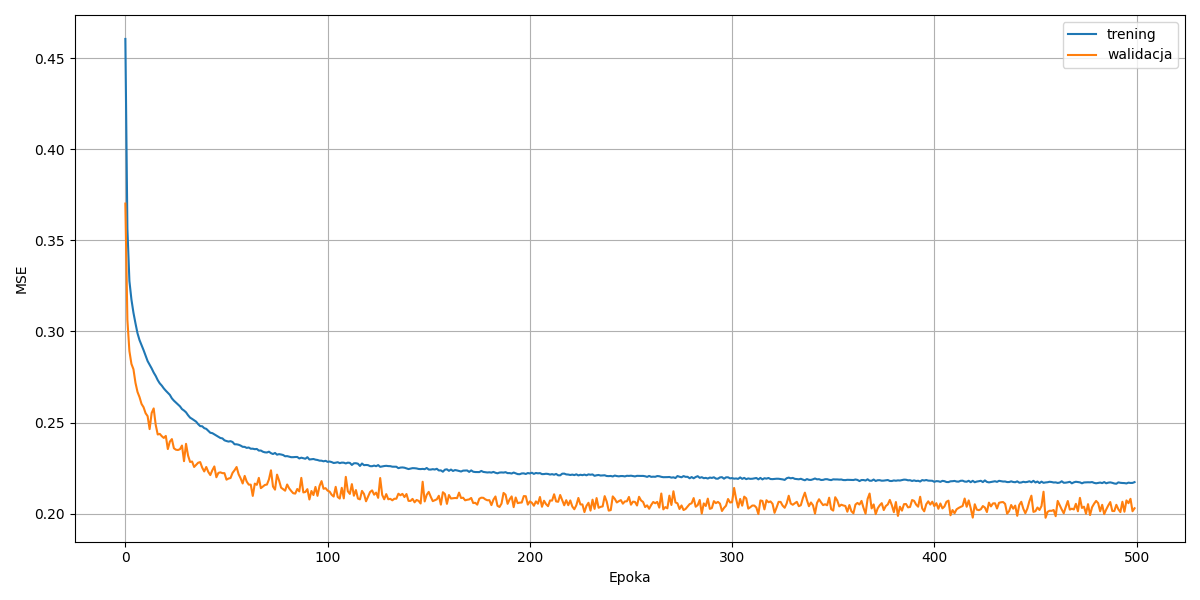
\includegraphics[width=1.0\textwidth]{./images/mae1_loss.png}
    \caption{Wartości funkcji kosztu MSE dla pierwszego samonadzorowanego treningu wstępnego}
    \label{fig:mae1_loss}
\end{figure}

% mae1 - loss
Na rysunku \ref{fig:mae1_loss} zaprezentowane zostały wartości funkcji kosztu na zbiorze treningowym i walidacyjnym w kolejnych epokach treningu. Najważniejszym wnioskiem jest to, że model się nie przetrenował. Druga obserwacja jest taka, że po zadanych $500$ epokach, wartość funkcji kosztu ciągle maleje, ale coraz wolniej. Szybkość spadania tych krzywych nie ma właściwie znaczenia, ponieważ to dopiero w późniejszym etapie treningu model zaczyna znajdować trudniejsze i bardziej złożone wzorce w danych treningowych. Nie prowadzą one jednak do tak gwałtownej poprawy wyników, jaka była możliwa na samym początku treningu, kiedy model znalazł najprostsze, przybliżone rozwiązanie --- interpolację stałą wartością między widocznymi fragmentami spektrogramów. Fakt, że wartość funkcji kosztu cały czas maleje świadczy o tym, że trening ten powininen trwać jeszcze dłużej, być może wielokrotnie dłużej. Ze względu na ograniczone zasoby i czas trzeba było jednak wprowadzić jakieś ograniczenie dla eksperymentów nienadzorowanych.

% mae1 - predykcje
Po każdej epoce zapisywane jest kilka przykładowych spektrogramów wejściowych i wyjściowych. Można na ich podstawie ocenić w jakim stopniu model rozumie przetwarzane dane i występujące w nich wzorce. Rysunek \ref{fig:mae1_predictions} pokazuje wybrane przykłady z opisywanego treningu nienadzorowanego. Przykłady pochodzą ze zbioru walidacyjnego po pierwszej, po około $10$, po około $100$ i po około $500$ epokach treningu. Pierwsza kolumna zawiera oryginalne dane wejściowa, w drugiej widoczne są jedynie te framenty, które wchodzą do enkodera, w trzeciej pokazane są predykcje dekodera.

\begin{figure}
    \centering
    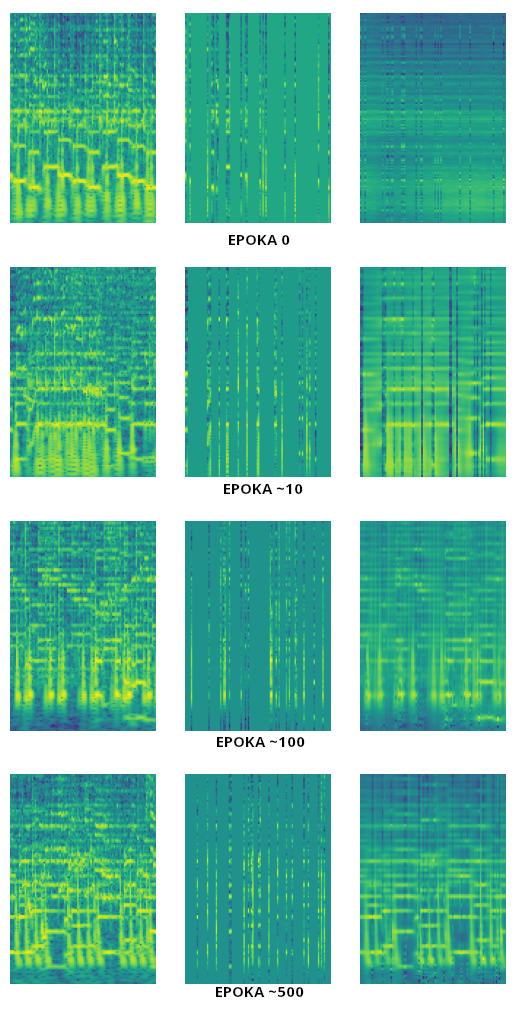
\includegraphics[width=0.8\textwidth]{./images/mae1_predictions.png}
    \caption{Predykcje modelu w trakcie pierwszego treningu nienadzorowanego.}
    \label{fig:mae1_predictions}
\end{figure}

% mae1 - predykcje
Jak widać na tym rysunku, po pierwszej epoce predykcje są praktycznie stałe, chociaż wyraźnie zależą od danych wejściowych. Jest to oczywiście pierwsze, najprostsze rozwiązanie, jakie może znaleźć model. W tym pierwszym spektrogramie wyjściowym widać również, że odznaczają się fragmenty, które nie były zamaskowane. Kontrast ten wynika być może częściowo z faktu, że funkcja kosztu jest przykładana jedynie do tokenów na pozycjach zamaskowanych.

% mae1 - predykcje
Po około $10$ widać już wyraźny postęp w nauce. Predykcje sieci są w ramach pojedynczego fragmentu znacznie bardziej zróżnicowane. Można powiedzieć, że przypomniają one już w znaczącym stopniu dane wejściowe, jeżeli skupić się na najsilniejszych częstotliwościach składowych. Na tym etapie należy jednak uznać, że model nie nauczył się jeszcze właściwie żadnych istotnych wzorców i reguł. Aby uzyskać zbliżony efekt uzupełniania wyciętych ramek, wystarczy wykonać prostą interpolację linową. W szczególności trzeba zwrócić uwagę, że jedynymi strukturami jakie pojawiają się w predykcji modelu są długie, dosyć rozmyte poziome linie.

% mae1 - predykcje
Po $100$ epokach wodel zdecydowanie jest już w stanie zlokalizować pewne powtarzające się wzorce we fragmencie utworu i uzupełnić je w brakujących miejscach. Widać to szczególnie w kontekście rytmu, ponieważ pojawiają się regularne akcenty, nawet wyraźniejsze niż w spektrogramie wejściowym. Wciąża jednak widać, że częst moment rozpoczęcia i zakończenia trwania pojedynczych tonów nie jest precyzyjnie określony (rozmyte linie). Po $500$ epokach predykcje stają się przede wszystkim ostrzejsze i precyzyjniejsze. Widać wyraźnie, to co występowało już po $100$ pokach: dłuższe dziury nie są uzupełniane stałymi wartościami, ale model uzupełnia w nich najbardziej prawdopodobne struktury.

% mae1 - predykcje
Ze względu na to, że ramki nie zostały pogrupowane w większe bloki i model dostaje dużo krótkich fragmentów z różnych chwil czasu, trudno ocenić, na jakim poziomie rzeczywiście rozumie przetwarzane dane. Zwłaszcza trudno to ocenić w kontekście struktur harmonicznych, ponieważ jeżeli chodzi o rytm, to wydaje się jasne, że sieć nauczyła się rozpoznawać rytm i uzupełniać odpowiednio akcenty w całym fragmencie utworu. Ta trudność w ocenie wynika z faktu, że maskowane są zawsze całe ramki, a pojedyncza ramka, choć nie zawiera żadnych informacji o rytmie, prezentuje właściwie komplet informacji na temat wysokości dźwięków z danej chwili czasu.

% mae1 - finetuning i wnioski
Tabela \ref{tab:results_medium-transformer-mae1-finetuning} prezentuje wyniki eksperymentu nadzorowanego, w którym model został zainicjowany parametrami z wytrenowanego w opisanym powyżej eksperymenc enkodera. Poza tym, wszystkie hiperparametry są takie same jak w poprzednim etapie. Różnica jest jednak widoczna w wynikach. Okazuje się, że \emph{poprzez samonadzorowany trening wstępny, uzyskane zostały lepsze wyniki klasyfikacji akordów}, niż w którymkolwiek z przeprowadzonych dotychczas eksperymentów nadzorowanych. Jednakże zdecydowanie niewielka przewaga w dokładności klasyfikacji nie jest tak istotna, jak fakt, że trzeba było kilkakrotnie mniej czasu, aby wynik ten osiągnąć. Zysk z pretreningu jest więc dwojaki: po pierwsze pozwala osiągnąć nieznacznie lepsze wyniki a po drugie pozwala osiągnać je znacznie szybciej. W niektórych przypadkach wystarczyło niecałe $20$ epok, aby zakończyć trening. Jeżeli chodzi o niewielki zysk w dokładności klasyfikacji, to wskazuje on po raz kolejny na to, że problemem są dane oznaczone. Prawdopodobnie wykorzystanie treningu nienadzorowanego jest w tym przypadku zdecydowanie nadmiarowe i aby usprawnić model rozpoznający akordy, należałoby skupić się na poprawieniu jakości danych, w tym również na lepszych metodach augmentacji, aby skuteczniej uniknąć przetrenowania.

\begin{table}
    \centering
    \caption{Hiperparametry i wyniki treningu \code{medium-transformer-mae1-finetuning}}
    \label{tab:results_medium-transformer-mae1-finetuning}
    \parbox{\textwidth}{\scriptsize\centering
    \vspace{20pt}
    \begin{tabular}{lc}
        \multicolumn{2}{c}{\textbf{HIPERPARAMETRY}} \\
        \hline \multicolumn{2}{c}{ZBIÓR DANYCH} \\ \hline
        \code{item\_mutliplier}         & $1$   \\
        \code{song\_multiplier}         & $20$   \\
        \code{augment}                  & TAK          \\
        \code{subsets}                  & None          \\
        \code{fraction}                 & $1.0$       \\
        \hline \multicolumn{2}{c}{MODEL} \\ \hline
        \code{model\_dim}               & $256$      \\
        \code{n\_heads}                 & $4$        \\
        \code{n\_blocks}                & $10$       \\
        \code{block\_type}              & transformer       \\
        \code{dropout\_p}               & $0.0$      \\
        \hline \multicolumn{2}{c}{TRENING} \\ \hline
        \code{n\_epochs}                & $2000$       \\
        \code{batch\_size}              & $500$     \\
        \code{lr}                       & $0.0005$             \\
        \code{early\_stopping}          & $50$ \\
    \end{tabular}
    \hspace{40pt}
    \begin{tabular}{ccc}
        \multicolumn{3}{c}{\textbf{WYNIKI OGÓLNE}} \\
        \hline Walidacja  & WCSR          & Liczba epok         \\ \hline
        1                 & $0.758$    & $18$    \\
        2                 & $0.767$    & $32$    \\
        3                 & $0.736$    & $20$    \\
        4                 & $0.75$    & $35$    \\
        5                 & $0.753$    & $37$    \\ \hline
        ŚREDNIA           & $\mathbf{0.753 \pm 0.01}$ & $\mathbf{28 \pm 8}$ \\ \hline
    \end{tabular}
    }
\end{table}



\section{Etap 5: Samonadzorowany trening wstępny --- drugie podejście}

% mae2 - hiperparametry
Ze względu na ograniczone zasoby i czas wykonany został jeszcze tylko jeden trening nienadzorowany. Różni się on od poprzedniego zasadą maskowania spektrogramów. Tym razem wycinanych było mniej ale dłuższych fragmentów --- $6$ ciągłych bloków po $10$ ramek z pojedynczego $100$-ramkowego fragmentu. Wydłużenie brakujących fragmentów ma zmusić model do głębszego wniknięcia i zrozumienia przetwarzanych utworów, które jest niezbędne, aby poprawnie uzupełnić dłuższe, zamaskowane ciągi ramek. Z drugiej strony, zmniejszenie proporcji maskowania ma uczynić to zadanie przede wszystkim wykonalnym. Wartości tych hiperparametrów nie były jednak dokładnie zbadane, ponieważ do tego trzeba by wykonać kilkadziesiąt pełnych treningów samonadzorowanych. Wybrana proporcja maskowania i liczba ramek w ciągłym bloku są więc głównie oparte na intuicji i prostych hipotezach, mogą więc okazać się jak najbardziej nieoptymalne. Poza tym, wszystkie pozostałe hiperparametry treningu są dokładnie takie same jak w poprzednim etapie, co widać w tabeli \ref{tab:params_mae2}.

\begin{table}
    \centering
    \caption{Hiperparametry drugiego treningu samonadzorowanego}
    \label{tab:params_mae2}
    {\scriptsize\begin{tabular}{lc}
        \multicolumn{2}{c}{ZBIÓR DANYCH} \\ \hline
        \code{item\_mutliplier} & $10$ \\
        \code{song\_multiplier} & $10$ \\
        \code{augment} & TAK \\
        \multicolumn{2}{c}{ENKODER} \\ \hline
        \code{encoder\_dim} & $256$ \\
        \code{encoder\_n\_heads} & $4$ \\
        \code{encoder\_n\_blocks} & $10$ \\
        \multicolumn{2}{c}{DEKODER} \\ \hline
        \code{decoder\_dim} & $256$ \\
        \code{decoder\_n\_heads} & $4$ \\
        \code{decoder\_n\_blocks} & $3$ \\
        \multicolumn{2}{c}{TRENING} \\ \hline
        \code{masking\_ratio} & $0.6$ \\
        \code{chunks\_per\_item} & $10$ \\
        \code{n\_epochs} & $500$ \\
        \code{batch\_size} & $100$ \\
        \code{lr} & $0.0002$ \\
    \end{tabular}}
\end{table}

\begin{figure}
    \centering
    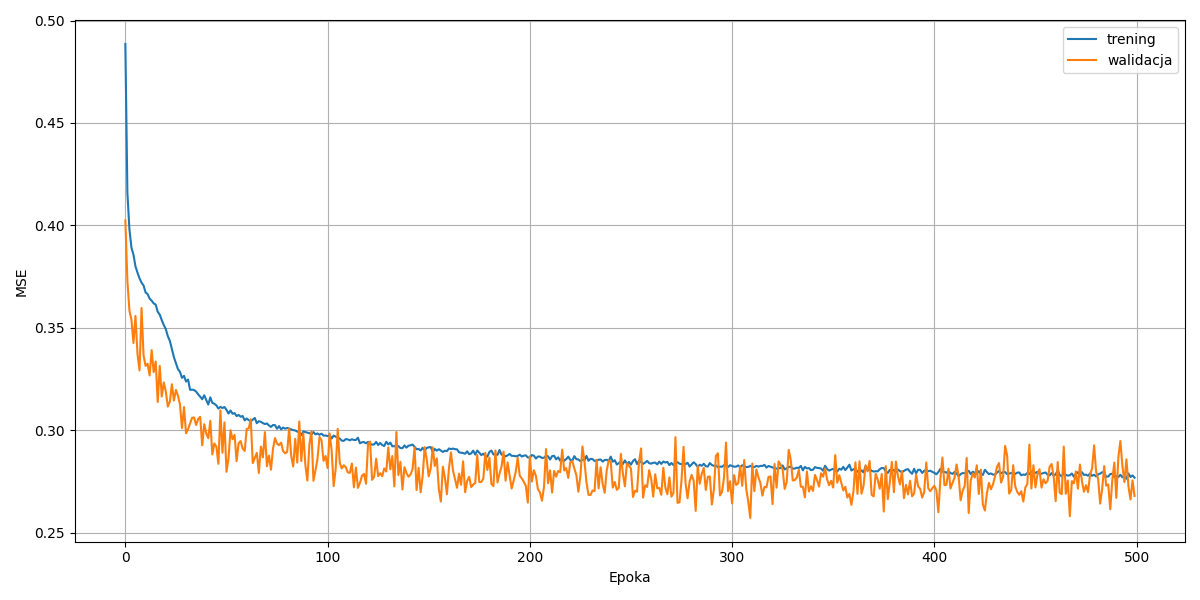
\includegraphics[width=1.0\textwidth]{./images/mae2_loss.png}
    \caption{Wartości funkcji kosztu MSE dla drugiego samonadzorowanego treningu wstępnego}
    \label{fig:mae2_loss}
\end{figure}

% mae2 - loss
Rysunek \ref{fig:mae2_loss} prezentuje wartości funkcji kosztu na zbiorze treningowym i walidacyjnym dla drugiego nienadzorowanego treningu wstępnego. Wykres ten różni się zdecydowanie od wykresu otrzymanego w poprzednim etapie. Po pierwsze wartości funkcji kosztu są wyższe i nie spadają tak gwałtownie w pierwszej części treningu. Oznacza to po prostu, że zadanie jest trudniejsze do nauczenia. Po drugie wariancja MSE na zbiorze walidacyjnym jest znacznie większa. Wynika to z faktu, że trafiają się w zbiorze walidacyjnym zarówno fragmenty, z którymi model radzi sobie dobrze, jak i takie, których nie potrafi tak precyzyjnie uzupełnić. Również jest to dobry znak, ponieważ jeżeli dziury są uzupełniane na podstawie szczegółowej analizy niezamaskowanych ramek, to powinny się trafiać zróżnicowane sytuacje, czasem trudniejsze a czasem łatwiejsze. Jeżeli model uzupełnia zamaskowane ramki na podstawie prostych statystyk, wtedy nie będzie miał znaczenia poziom złożoności danego utworu. Celem zaś treningu wstępnego jest nauczyć model złożony zależności obecnych w utworach muzycznych. Ostatnią obserwacją dotyczącą tych krzywych jest zbliżenie się wartości na zbiorze walidacyjnym do wartości na zbiorze treningowym w końcowej części treningu. Sugeruje to potencjalne przetrenowanie, ale nie jest to jeszcze pewne na tym etapie. Być może po prostu jakość predykcji na zbiorze walidacyjnym i treningowym zrównają się i dalej będą malały. Podobnie jak w poprzednim etapie trening ten powinen trwać dłużej, jeżeli by to było możliwe.

\begin{figure}
    \centering
    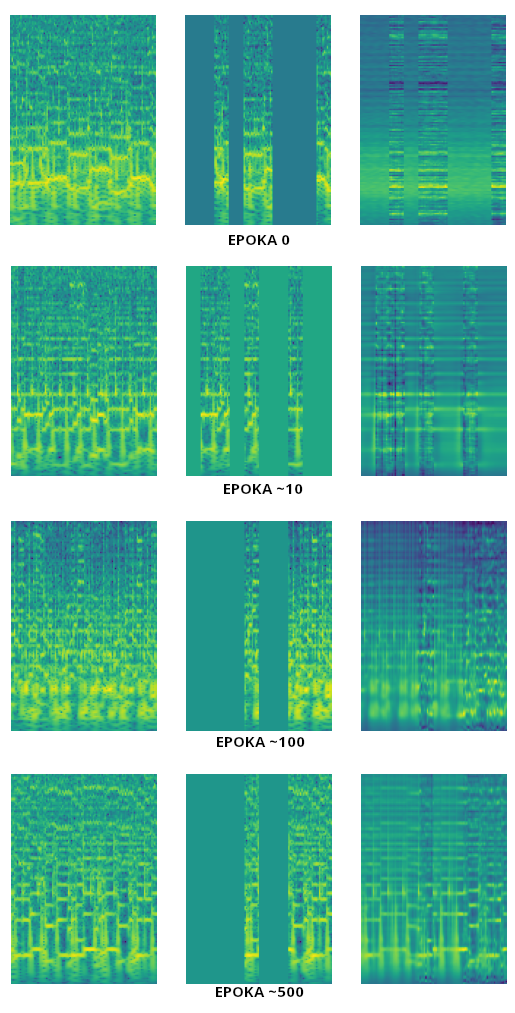
\includegraphics[width=0.8\textwidth]{./images/mae2_predictions.png}
    \caption{Predykcje modelu w trakcie drugiego treningu nienadzorowanego.}
    \label{fig:mae2_predictions}
\end{figure}

% mae2 - predykcje
Na rysunku \ref{fig:mae2_predictions} widać przykładowe predykcje na zbiorze walidacyjnym, po pierwszej, po około $10$, po około $100$ i po około $500$ epokach treningu. Z powodu zmiany parametrów maskowania, wycinane fragmenty to duże, często stojące obok siebie bloki. Sytuacja po pierwszej epoce jest praktycznie taka sama jak w poprzednim etapie. Model zwraca stałe wartości, dla zamaskowanych ramek. Różnice w obu treningach samonadzorowanych zaczynają być jednak widoczne już po $10$ epokach. Dokładność uzupełniania dziur jest tym razem zdecydowanie gorsza. Widać wyraźnie, że model ,,rozciąga'' ramki z brzegów niezamaskowanych fragmentów --- wykonuje interpolację liniową. Taka sama metoda daje znacznie lepszy efekt, kiedy jest nawet więcej, ale małych ubytków w spektrogramie.

% mae2 - predykcje
Po $100$ epokach zaczyna być widać zdolność modelu do wyszukiwania bardziej złożonych zależności. Zaczął on rozpoznawać rytm, wyraźnie dodająć równe akcenty w całym wytwarzanym spektrogramie. Widać też, że potrafi uzupełnić dłuższe, ale regularne struktury. Właściwości te wzmacniają się w dalszej części treningu i po $500$ epokach można obserwować nieraz całkiem (choć nie za bardzo) spektakularne domysły sieci neuronowej. Na przedstawionym rysunku widać, że model uzupełnił pierwszy, dłuższy z dwóch zamaskowanych fragmentów. Pomylił się jednak i drugi, wyższy dźwięk, rozciągnął zbyt długo. Można przypuszczać, że założył najprostszy możliwy schemat, który powtórzony wpasuje się dobrze w widoczne fragmenty spektrogramu. 

% mae2 - predykcje (refleksja)
Dzięki zmianie w sposobie maskowania w tym drugim treningu samonadzorowanym, łatwiej można ocenić zasady działania modelu. Oglądajęc jego predykcje, trudno nazwać je twórczymi i utworzonymi w wyniku znalezienia bardziej złożonych zależności. Wydają się one sprowadzać do kopiowania tego co nie jest zamaskowane i odpowiedniego rozmieszczenia w czasie. Trudno tak naprawdę dobrze to ocenić. Należy jednak pamiętać, że jest to tylko etap pośredni, mający na celu wyuczenie dobrego ekstraktora cech. Nie jest w gruncie rzeczy ważne, czy zadanie wstępne, jakim jest w tym przypadku uzupełnienie fragmentów spektrogramu, będzie wykonane dobrze. Dlatego też właściwym sposobem sprawdzenia użyteczności tego drugiego podejścia do trenigu samonadzorowanego jest, tak jak w poprzednim etapie, dotrenowanie enkodera na zadaniu rozpoznawania akordów. Gdyby celem było tworzenie dobrej jakości muzyki, należałoby uciec się do zupełnie innych metod, przystosowanych do zadań generowania treści.

% mae2 - finetuning
Wyniki dotrenowania enkodera na zadaniu rozpoznawania akordów przedstawione są w tabeli \ref{tab:results_medium-transformer-mae2-finetuning}. Ze względu na większy poziom trudności zadania wstępnego, można się było spodziewać, że zysk przy dotrenowaniu będzie większy. Jeżeli chodzi o dokładność klasyfikacji to okazuje się ona nieznacznie niższa niż w przypadku poprzedniego dotrenowania, choć wciąż wyższa niż dokładnośc modeli uczonych od zera. Można powtórzyć tutaj, że dokładność ta nie ma specjalnego znaczenia. Istotny natomiast jest fakt, że dotrenowanie trwało w tym przypadku jeszcze krócej, niż w poprzednim etapie. Trudno powiedzieć, czy jest to wynik losowy czy spowodowany lepszymi wagami początkowymi. 

% mae2 vs mae1 i wnioski
Zysk z obu wstępnych treningów samonadzorowanych wbrew oczekiwaniom wydaje się być podobny. Nie można jednak dobrze ocenić, czy oznacza to, że uzyskane enkodery dokonują ekstrakcji cech na podobnym poziomie. Jak już wielokrotnie wspominano, wyniki na zadaniu rozpoznawania akordów są mocno ograniczone przez jakość danych uczących. To jest pierwsza potencjalna przyczyna nie uwidocznienia się różnić w zysku z obu pretreningów. Druga potencjalna, i na dodatek dość prawdopodbna przyczyna jest taka, że dekodery były zbyt duże. Nie przeprowadzono bowiem żadnych eksperymentów z mniejszymi dekoderami, które wymuszałyby agregację większej ilości informacji w enkoderze. Tak naprawdę, mogą być one równie dobrze zbyt małe, chociaż ten kierunek nie wydaje się być zgodny z intuicją, ponieważ trenowane modele i tak są już zdecydowanie większe, niż potrzeba do zadania rozpoznawania akordów \cite{ohanlon_fifthnet_2021}. W każdym razie, możliwe że enkodery realizują tylko jakieś proste normalizacje danych wejściowych a całość zadania uzupełniania zamaskowanych ramek wykonuje dekoder. Niestety dostępne zasoby sprzętowe i czasowe nie pozwoliły na dokładne zbadanie tego tematu. Faktem pozostaje, że treningi wstępne, które wykonano w ramach niniejszej pracy, dają duży zysk w czasie treningu nadzorowanego i wydaje się nie być stratą czasu przeprowadzanie kolejnych, bardziej szczegółowych eksperymentów w tym temacie (ale ja mam już dość na razie).

\begin{table}
    \centering
    \caption{Hiperparametry i wyniki treningu \code{medium-transformer-mae2-finetuning}}
    \label{tab:results_medium-transformer-mae2-finetuning}
    \parbox{\textwidth}{\scriptsize\centering
    \vspace{20pt}
    \begin{tabular}{lc}
        \multicolumn{2}{c}{\textbf{HIPERPARAMETRY}} \\
        \hline \multicolumn{2}{c}{ZBIÓR DANYCH} \\ \hline
        \code{item\_mutliplier}         & $1$   \\
        \code{song\_multiplier}         & $20$   \\
        \code{augment}                  & TAK          \\
        \code{subsets}                  & None          \\
        \code{fraction}                 & $1.0$       \\
        \hline \multicolumn{2}{c}{MODEL} \\ \hline
        \code{model\_dim}               & $256$      \\
        \code{n\_heads}                 & $4$        \\
        \code{n\_blocks}                & $10$       \\
        \code{block\_type}              & transformer       \\
        \code{dropout\_p}               & $0.0$      \\
        \hline \multicolumn{2}{c}{TRENING} \\ \hline
        \code{n\_epochs}                & $2000$       \\
        \code{batch\_size}              & $500$     \\
        \code{lr}                       & $0.0005$             \\
        \code{early\_stopping}          & $50$ \\
    \end{tabular}
    \hspace{40pt}
    \begin{tabular}{ccc}
        \multicolumn{3}{c}{\textbf{WYNIKI OGÓLNE}} \\
        \hline Walidacja  & WCSR          & Liczba epok         \\ \hline
        1                 & $0.756$    & $20$    \\
        2                 & $0.767$    & $22$    \\
        3                 & $0.733$    & $16$    \\
        4                 & $0.744$    & $22$    \\
        5                 & $0.748$    & $11$    \\ \hline
        ŚREDNIA           & $\mathbf{0.75 \pm 0.012}$ & $\mathbf{18 \pm 4}$ \\ \hline
    \end{tabular}
    }
\end{table}



\section{Etap 6: Samonadzorowany trening wstępny --- pierwsze podejście}
